\begin{frame}
\frametitle{Примитивная задача планирования}

Список задач (даже пока не потоков) дан заранее:
\begin{itemize}
  \item<2-> про каждую задачу известна ее длительность;
  \item<3-> задача работает от начала и до конца (не прерываясь, не вытесняясь);
  \item<4-> какой смысл вообще что-то придумывать в такой ситуации?
\end{itemize}
\end{frame}

\begin{frame}
\frametitle{Пример}

\begin{columns}[T]
  \begin{column}{.4\textwidth}
    \begin{figure}
      \centering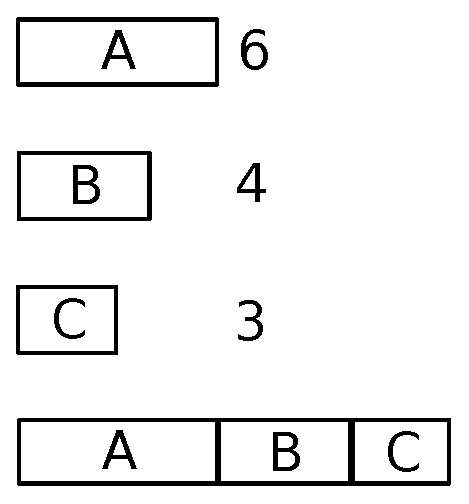
\includegraphics[width=.9\linewidth]{sched0}
      \caption{Example Schedule}
    \end{figure}
  \end{column}
  \begin{column}{.6\textwidth}
    \begin{itemize}
      \item<2-> $TOTAL = 6 + 4 + 3 = 13$
      \item<3-> $WAIT_A = 6$
      \item<3-> $WAIT_B = 6 + 4 = 10$
      \item<3-> $WAIT_C = 6 + 4 + 3 = 13$
      \item<4-> $WAIT_{AVG} = {\left(6 + 10 + 13\right)\over 3} = 9.\left(6\right)$
    \end{itemize}
  \end{column}
\end{columns}
\end{frame}

\begin{frame}
\frametitle{Пример}

\begin{columns}[T]
  \begin{column}{.4\textwidth}
    \begin{figure}
      \centering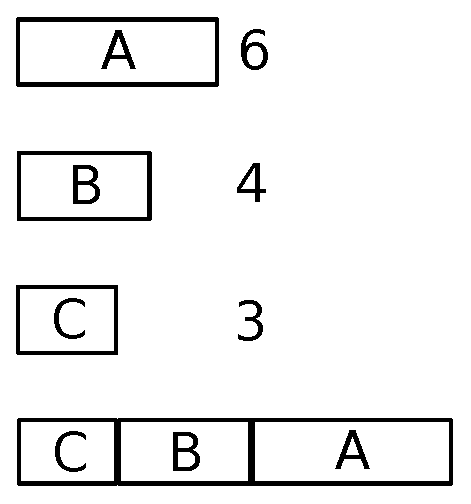
\includegraphics[width=.9\linewidth]{sched1}
      \caption{Example Schedule}
    \end{figure}
  \end{column}
  \begin{column}{.6\textwidth}
    \begin{itemize}
      \item<2-> $TOTAL = 6 + 4 + 3 = 13$
      \item<3-> $WAIT_C = 3$
      \item<3-> $WAIT_B = 3 + 4 = 7$
      \item<3-> $WAIT_A = 6 + 4 + 3 = 13$
      \item<4-> $WAIT_{AVG} = {\left(3 + 7 + 13\right)\over 3} = 7.\left(6\right)$
    \end{itemize}
  \end{column}
\end{columns}
\end{frame}

\begin{frame}
\frametitle{Shortes Job First}

Shortest Job First (SJF) - гарантирует минимальное \emph{среднее} время ожидания завершения задачи.

\onslide<2>{\emph{Доказательство:} ну это же очевидно!}
\end{frame}

\begin{frame}
\frametitle{Shortes Job First}

\emph{Доказательство:}
\begin{itemize}
  \item планируем $N$ задач, с временами работы $T_0$, $T_1$, ..., $T_{N-1}$;
  \item допустим, что в расписании с наименьшим $WAIT_{AVG}$ есть две
        задачи $s$ и $t$, такие что $T_s > T_t$, но $s$ идет раньше чем $t$;
  \item поменяем местами $s$ и $t$ в расписании;
  \item все задачи до $t$ и начиная с $s$ имеют тоже самое время ожидания;
  \item все задачи начиная с $t$ и до $s$ имеют меньшее время ожидания;
  \item получили расписание с меньшим $WAIT_{AVG}$ - противоречие.
\end{itemize}
\end{frame}

\begin{frame}
\frametitle{Ввод и вывод}

\begin{itemize}
  \item<1-> задачи могут обращаться к медленным внешним устройствам или ждать
            внешних событий:
              \begin{itemize}
                \item задача, которая только ждет - бесполезно занимает
                      процессор (естественная точка перепланирования);
              \end{itemize}
  \item<2-> задачу стоит снять с процессора:
     \begin{itemize}
       \item если задача не критична к времени отклика, то стоит использовать
             прерывания;
       \item если внешнее устройство обрабатывает запросы долго, то стоит
             использовать прерывания;
       \item если время ожидания не предсказуемо (получение пакета по сети или
             ожидание нажатия клавиши), то стоит использовать прерывания;
     \end{itemize}
\end{itemize}
\end{frame}

\begin{frame}
\frametitle{Пример}

\begin{columns}[T]
  \begin{column}{.4\textwidth}
    \begin{figure}
      \centering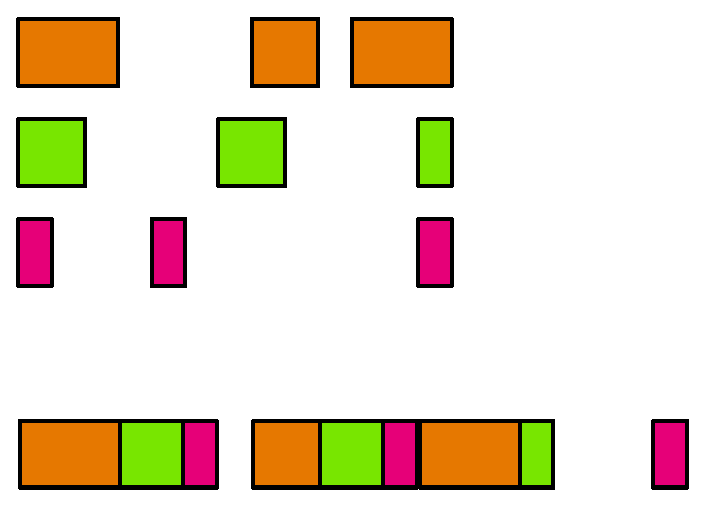
\includegraphics[width=1.0\linewidth]{iosched0}
      \caption{Schdeule with IO}
    \end{figure}
  \end{column}
  \begin{column}{.6\textwidth}
    \begin{itemize}
      \item в расписании могут появляться "дыры" (все ждут завершения IO)
      \item интуиция - хотим, максимально параллельный IO:
        \begin{itemize}
          \item реалистично для сети или клавиатуры;
          \item не реалистично, например, для диска - общий ресурс.
        \end{itemize}
    \end{itemize}
  \end{column}
\end{columns}
\end{frame}

\begin{frame}
\frametitle{Пример}

\begin{columns}[T]
  \begin{column}{.4\textwidth}
    \begin{figure}
      \centering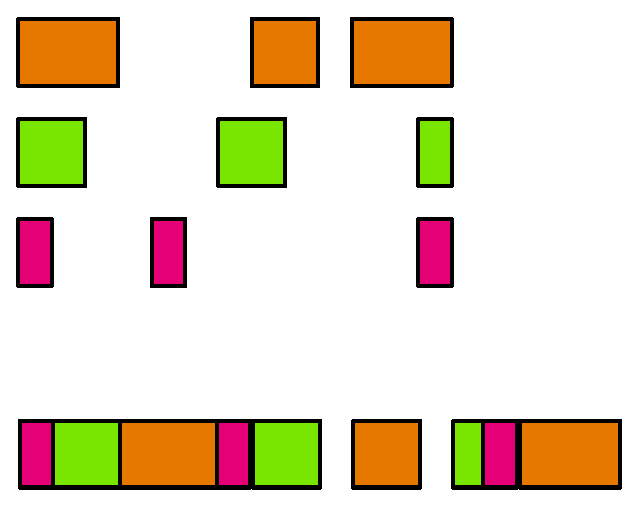
\includegraphics[width=1.0\linewidth]{iosched1}
      \caption{Schdeule with IO}
    \end{figure}
  \end{column}
  \begin{column}{.6\textwidth}
    \begin{itemize}
      \item задачу с ближайшим IO пропускаем вперед:
        \begin{itemize}
          \item чем раньше задача начнет IO, тем лучше;
          \item чем больше задач будет выполнять IO параллельно, тем лучше;
          \item при прочих равных, задачу с большим IO стоит пустить раньше;
          \item получаем SJF с учетом IO;
        \end{itemize}
    \end{itemize}
  \end{column}
\end{columns}
\end{frame}

\begin{frame}
\frametitle{Ограничения}

\begin{itemize}
  \item<1-> мы не знаем заранее время до следующего IO (или завершения)
        \begin{itemize}
          \item мы можем его примерно оценить основывась на "истории" работы
                задачи;
        \end{itemize}
  \item<2-> список задач не дан заранее
        \begin{itemize}
          \item SJF теряет свою оптимальность в этом случае (трудно планировать
                без полной информации и без возможности изменить решение);
          \item для оптимального планирования нам нужно вытеснять задачи в
                произвольные моменты времени (вытесняющая многозадачность);
        \end{itemize}
  \item<3-> IO зависит от внешних условий (пользователь, нагрузка, другие
            задачи);
\end{itemize}
\end{frame}

\begin{frame}
\frametitle{Round Robin}

Сделаем ограничения более реалистичными (переходим от задач к потокам):
\begin{itemize}
  \item<1-> мы можем снимать поток с процессора в любое время (не спрашивая
        разрешения у потока):
        \begin{itemize}
          \item когда задача запускает операцию ввода/вывода;
          \item по сигналу от таймера;
        \end{itemize}
  \item<2-> больше мы ничего не знаем о потоке.
\end{itemize}
\end{frame}

\begin{frame}
\frametitle{Round Robin}

Если мы ничего не знаем о потоках - дадим каждому по чуть-чуть по очереди:
\begin{itemize}
  \item<2-> нужно ограничить время работы на процессоре (квант времени)
        \begin{itemize}
          \item поток может "заблокироваться" раньше, чем истечет квант времени;
        \end{itemize}
  \item<3-> все активные потоки выполняются по очереди
        \begin{itemize}
          \item если поток отработал квант, ставим его в конец очереди;
          \item если поток "разблокировался", ставим его в конец очереди;
        \end{itemize}
  \item<4-> Round Robin дает гарантии реального времени:
        \begin{itemize}
          \item зная, сколько всего потоков мы можем посчитать максимальное
                время ожидания;
        \end{itemize}
\end{itemize}
\end{frame}

\begin{frame}
\frametitle{Что не так с Round Robin?}

Рассмотрим планирование нескольких задач из двух классов:
\begin{enumerate}
  \item<2-> CPU bounded - не блокируются, постоянно вырабатывают свой квант:
        \begin{itemize}
          \item например, какие-то численные расчеты попадают в этот класс;
        \end{itemize}
  \item<3-> IO bounded - работают мало, ждут долго - не вырабатывают свой квант:
        \begin{itemize}
          \item например, текстовый редактор большую часть времени ждет ввода;
        \end{itemize}
\end{enumerate}
\end{frame}

\begin{frame}
\frametitle{Что не так с Round Robin?}
\begin{figure}
  \only<1>{\centering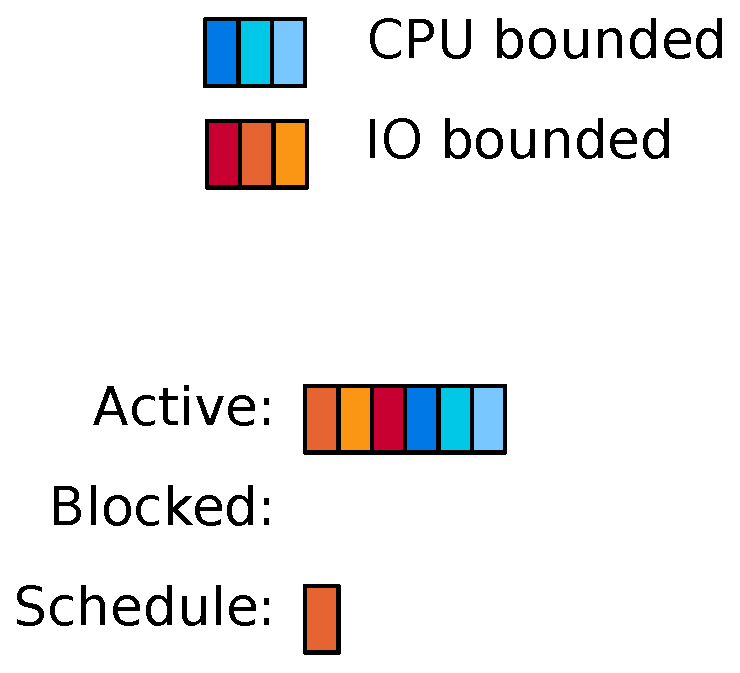
\includegraphics[width=.6\linewidth]{rr0}}
  \only<2>{\centering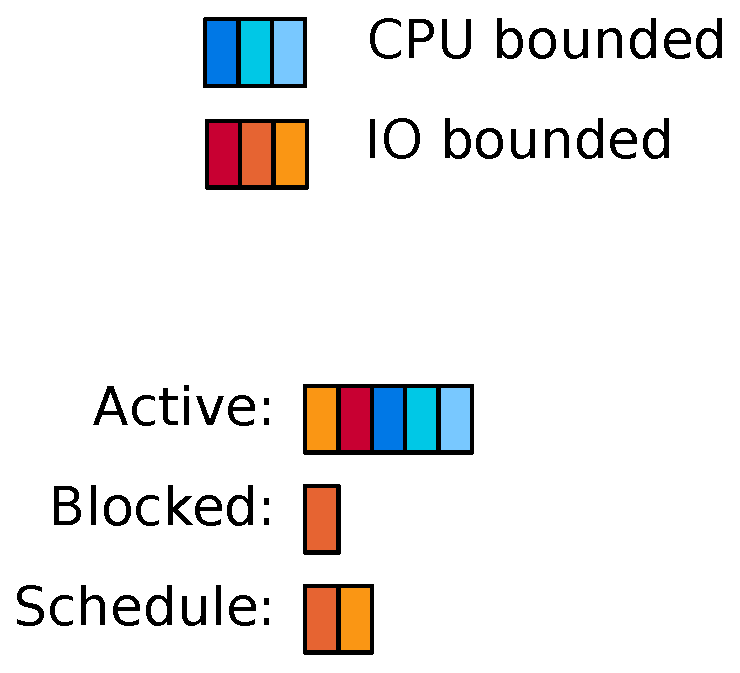
\includegraphics[width=.6\linewidth]{rr1}}
  \only<3>{\centering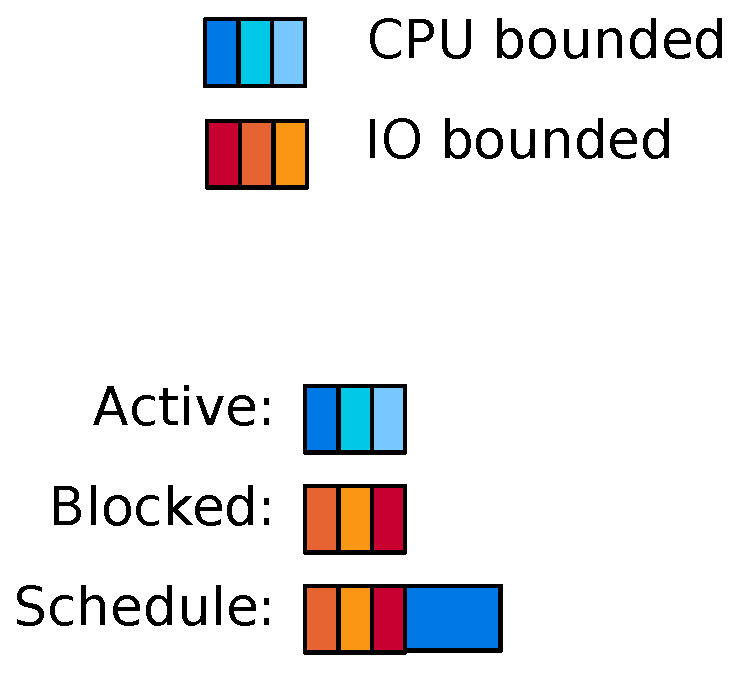
\includegraphics[width=.6\linewidth]{rr2}}
  \only<4>{\centering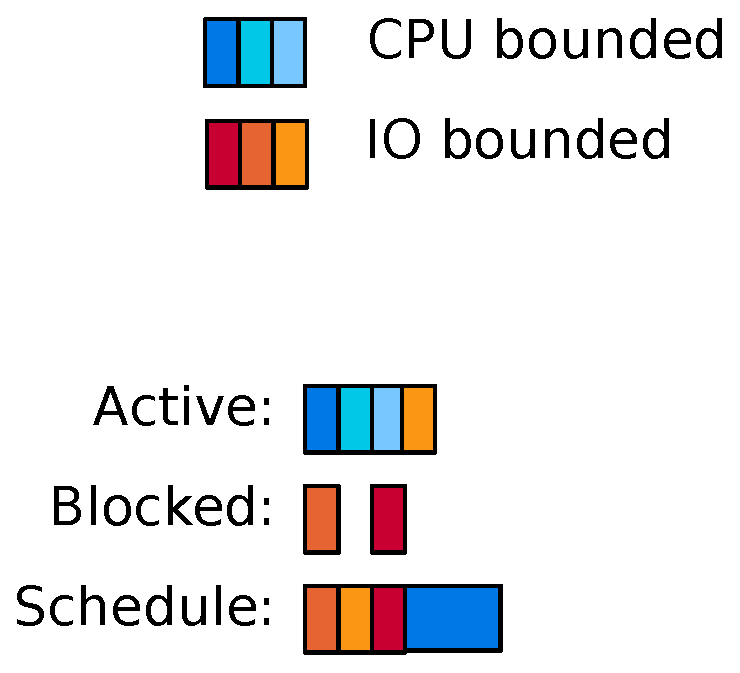
\includegraphics[width=.6\linewidth]{rr3}}
  \only<5>{\centering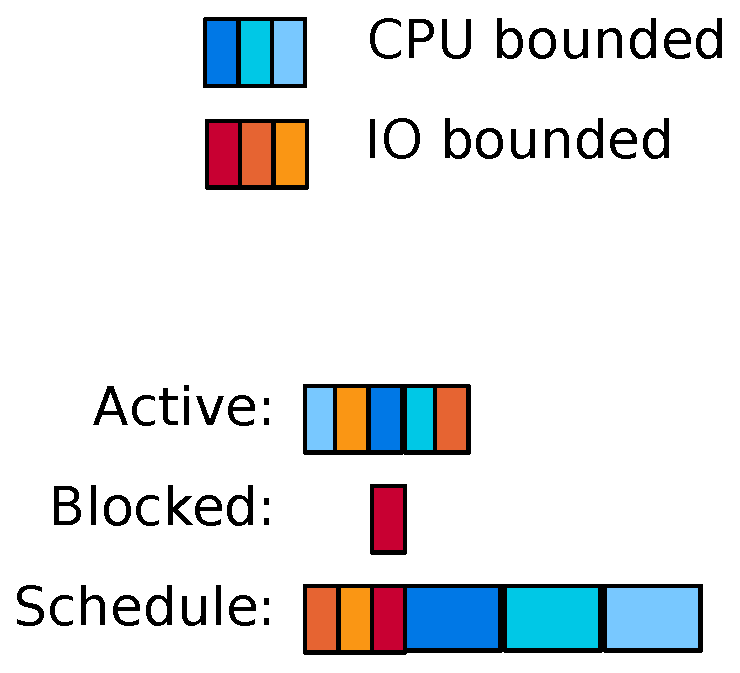
\includegraphics[width=.7\linewidth]{rr4}}
  \only<6>{\centering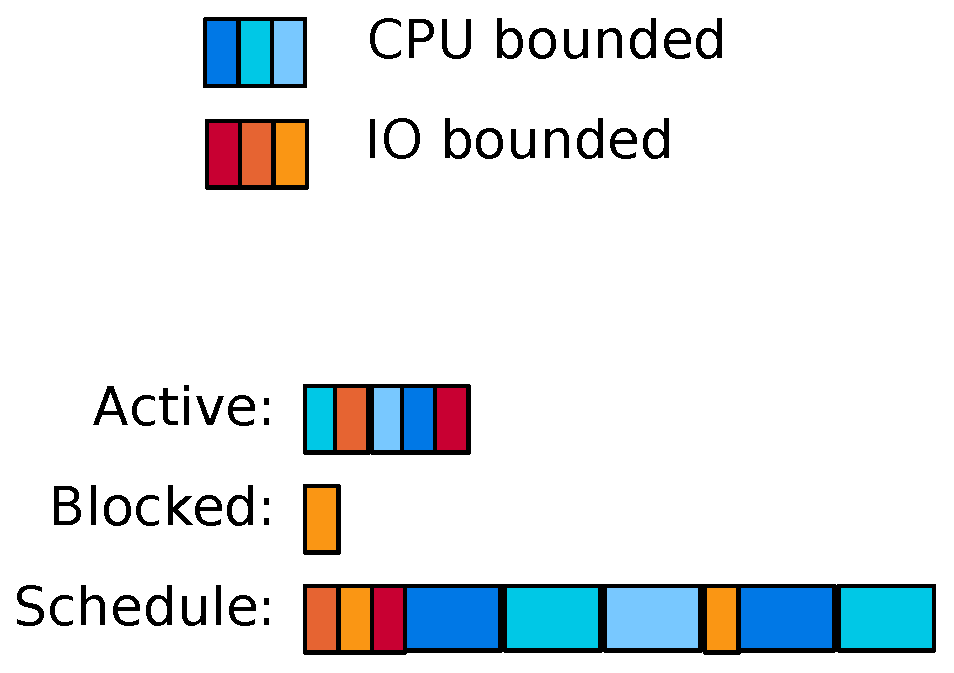
\includegraphics[width=.7\linewidth]{rr5}}
  \only<7>{\centering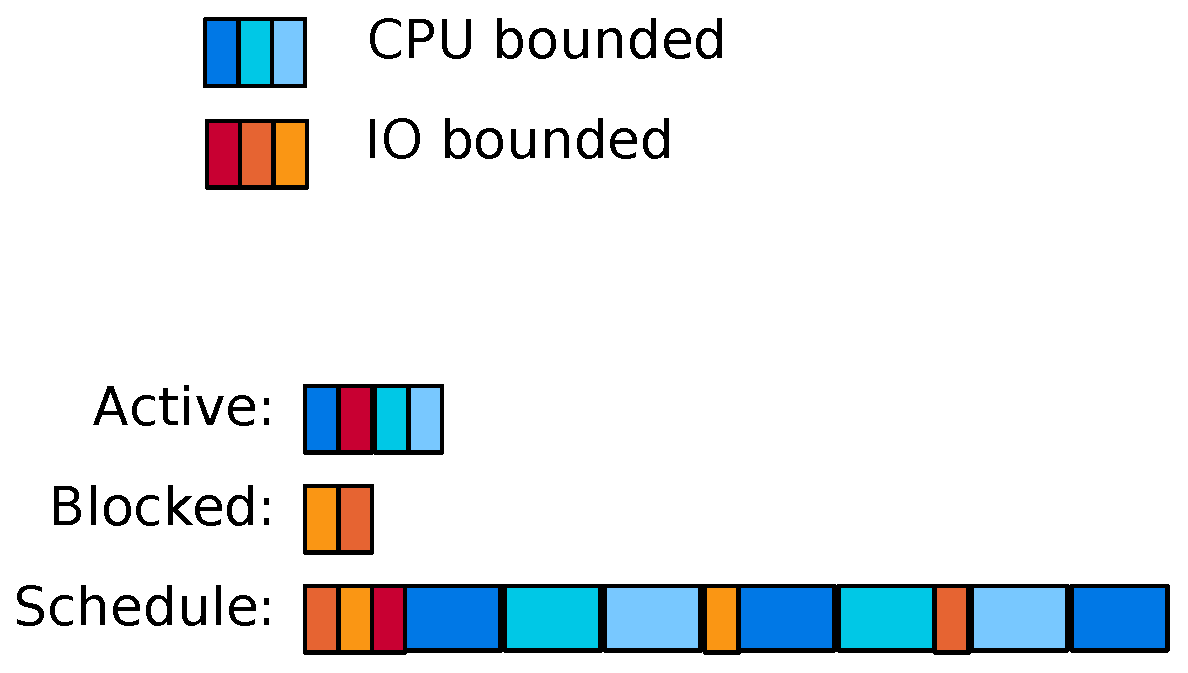
\includegraphics[width=.8\linewidth]{rr6}}
  \only<8>{\centering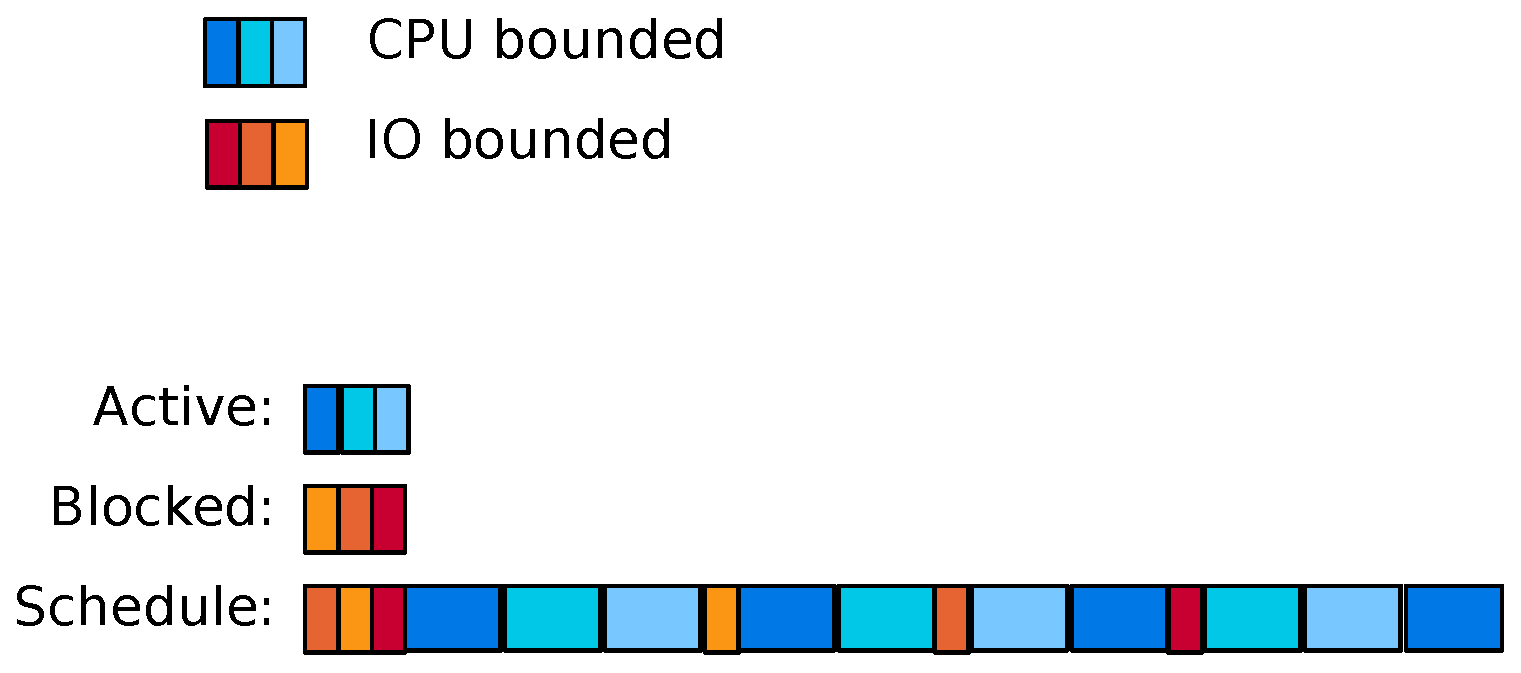
\includegraphics[width=.9\linewidth]{rr7}}
  \caption{Round Robin Example}
\end{figure}
\end{frame}

\begin{frame}
\frametitle{Что не так с Round Robin?}

\begin{itemize}
  \item<1-> IO bounded потоки получают много меньше CPU, а ждут столько же:
    \begin{itemize}
      \item это кажется не честным;
      \item IO bounded потоки - это, часто, интерактивные потоки (т. е.
            пользователь не доволен);
    \end{itemize}
  \item<2-> нужна возможность учитывать разные классы задач:
    \begin{itemize}
      \item в примере мы могли ставить IO bounded задачи в начало (осторожно,
            может приводить к старвации!);
      \item приоритезация задач:
            \begin{itemize}
              \item IO bounded vs CPU bounded;
              \item внутри класса можно варьировать квант времени;
            \end{itemize}
    \end{itemize}
\end{itemize}
\end{frame}
